\documentclass[12pt,oneside, reqno]{report}
\usepackage{pgfplots} 
\usepackage[utf8]{inputenc}
\usepackage{a4}
\usepackage{hyperref}
\usepackage[none]{hyphenat} %hyphenation
\sloppy
\usepackage{parskip} %no indentation after paragraphs
\usepackage{umlaute}
\usepackage{afterpage} %for using \afterpage{\clearpage} (don't push images to the end of a chapter)
\usepackage{makeidx}
\usepackage[numbers]{natbib}
\usepackage{graphicx}
\usepackage{picins} %provides precise control over the placement of inline graphics
\usepackage{setspace}
\usepackage{titlesec}
\usepackage{dsfont} %math symbols
\usepackage{tabularx}
\usepackage{floatflt} %float text around figures and tables
% Florian Schulze, 06.06.2012
% v1.0, latest edit: 06.06.2012

\usepackage[acronym]{glossaries}

\usepackage{enumitem} %resume counting from previous enumerate block
\usepackage{amsmath,amssymb}
\usepackage[format=default,font=footnotesize,labelfont=bf]{caption}
\usepackage{listings} %for listing source code
\usepackage{color}
\usepackage{algpseudocode} %for listing pseudocode
\usepackage{algorithm} %wrap algpseudocode and enrich with label etc.
\usepackage{float} % for [H] after floats


\graphicspath{{C:/Users/Kevin/Bachelarbeit/Bachelorarbeit/01_Bachelorarbeit_LaTex/02_Figures/}}

%\graphicspath{{/home/ga96jul/Bachelarbeit/Bachelorarbeit/01_Bachelorarbeit_LaTex/02_Figures/}}

\titleformat{\paragraph}[hang]{\normalfont\bfseries}{\theparagraph}{.5em}{}

\makeindex
\frenchspacing
\sloppy

\pagestyle{headings}

\textwidth16cm
\textheight22cm

\topmargin0cm
\oddsidemargin0cm
\evensidemargin0cm

\newcommand\boldred[1]{\textcolor{red}{\textbf{#1}}}

\newcommand{\bildklein}[3]{  
	\begin{figure}[hp]
	\begin{center}
	\includegraphics[width=0.5\textwidth]{#1}
	\end{center}
	\caption[#2]{#3}
	\end{figure}
}
  	
\newcommand{\bildgross}[3]{  
	\begin{figure}[hp]
	\begin{center}
	\includegraphics[width=0.95\textwidth]{#1}
	\end{center}
	\caption[#2]{#3}
	\end{figure}
}
  

\newcommand{\eqn}[3]{
	\begin{figure}[hp]
	\begin{equation}#1\end{equation}
	\caption[#2]{#3}
	\end{figure}
}

% This is tumlogo.tex
%
% Neues TUM-Logo in TeX
%   by G. Teege, 19.10.89
% Benutzung:
%   Am Anfang des Dokuments (TeX oder LaTeX):
%     \input tumlogo
%   Dann beliebig oft:
%     \TUM{<breite>}
%   bzw.
%     \oTUM{<breite>}
%   \TUM setzt das Logo mit der Breite <breite> und der entsprechenden Hoehe.
%   <breite> muss eine <dimen> sein. \oTUM erzeugt eine "outline"-Version
%   des Logos, d.h. weiss mit schwarzem Rand. Bei \TUM ist es ganz schwarz.
%   \oTUM entspricht damit der offiziellen Version des Logos.
%   Das Logo kann wie ein einzelnes Zeichen verwendet werden.
%   Beispiel:
%     Dies ist das TUM-Logo: \oTUM{1cm}.
%
\def\TUM#1{%
\dimen1=#1\dimen1=.1143\dimen1%
\dimen2=#1\dimen2=.419\dimen2%
\dimen3=#1\dimen3=.0857\dimen3%
\dimen4=\dimen1\advance\dimen4 by\dimen2%
\setbox0=\vbox{\hrule width\dimen3 height\dimen1 depth0pt\vskip\dimen2}%
\setbox1=\vbox{\hrule width\dimen1 height\dimen4 depth0pt}%
\setbox2=\vbox{\hrule width\dimen3 height\dimen1 depth0pt}%
\setbox3=\hbox{\copy0\copy1\copy0\copy1\box2\copy1\copy0\copy1\box0\box1}%
\leavevmode\vbox{\box3}}
%
\def\oTUM#1{%
\dimen1=#1\dimen1=.1143\dimen1%
\dimen2=#1\dimen2=.419\dimen2%
\dimen3=#1\dimen3=.0857\dimen3%
\dimen0=#1\dimen0=.018\dimen0%
\dimen4=\dimen1\advance\dimen4 by-\dimen0%
\setbox1=\vbox{\hrule width\dimen0 height\dimen4 depth0pt}%
\advance\dimen4 by\dimen2%
\setbox8=\vbox{\hrule width\dimen0 height\dimen4 depth0pt}%
\advance\dimen4 by-\dimen2\advance\dimen4 by-\dimen0%
\setbox4=\vbox{\hrule width\dimen4 height\dimen0 depth0pt}%
\advance\dimen4 by\dimen1\advance\dimen4 by\dimen3%
\setbox6=\vbox{\hrule width\dimen4 height\dimen0 depth0pt}%
\advance\dimen4 by\dimen3\advance\dimen4 by\dimen0%
\setbox9=\vbox{\hrule width\dimen4 height\dimen0 depth0pt}%
\advance\dimen4 by\dimen1%
\setbox7=\vbox{\hrule width\dimen4 height\dimen0 depth0pt}%
\dimen4=\dimen3%
\setbox5=\vbox{\hrule width\dimen4 height\dimen0 depth0pt}%
\advance\dimen4 by-\dimen0%
\setbox2=\vbox{\hrule width\dimen4 height\dimen0 depth0pt}%
\dimen4=\dimen2\advance\dimen4 by\dimen0%
\setbox3=\vbox{\hrule width\dimen0 height\dimen4 depth0pt}%
\setbox0=\vbox{\hbox{\box9\lower\dimen2\copy3\lower\dimen2\copy5%
\lower\dimen2\copy3\box7}\kern-\dimen2\nointerlineskip%
\hbox{\raise\dimen2\box1\raise\dimen2\box2\copy3\copy4\copy3%
\raise\dimen2\copy5\copy3\box6\copy3\raise\dimen2\copy5\copy3\copy4\copy3%
\raise\dimen2\box5\box3\box4\box8}}%
\leavevmode\box0}
% End of tumlogo.tex



\begin{document}
\nocite{*} %include uncited references in bibliography
\hoffset=5mm
\thispagestyle{empty}

\begin{center}
	\bigskip \bigskip \bigskip 
	\oTUM{6.0cm} \\
	\vspace*{0.8cm}
	{\huge \bf Technische Universität} \\
	\bigskip
	{\huge \bf München} \\
	\bigskip \bigskip \bigskip
	{\huge \bf Fakultät für Informatik} \\
	\bigskip \bigskip \bigskip
	{\Large \bf Master's Thesis in Informatik} \\
	\bigskip \bigskip \bigskip \bigskip \bigskip
	{\Large An Email-Centered Approach to Intelligent Task Management Using Crowdsourcing and Natural Language Processing} \\        
	\bigskip \bigskip \bigskip \bigskip
	{\Large John Doe} \\    
	\bigskip
	\begin{figure}[ht]
	\centering 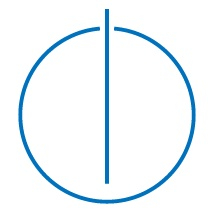
\includegraphics[width=0.2\linewidth]{figures/infologo.jpg}
	\end{figure}
	\bigskip 
\end{center}

\vfill

\newpage
\hoffset=5mm
\thispagestyle{empty}

\begin{center}
	\bigskip \bigskip \bigskip 
	\oTUM{6.0cm} \\
	\vspace*{0.8cm}
	{\huge \bf Technische Universität} \\
	\bigskip
	{\huge \bf München} \\
	\bigskip \bigskip \bigskip
	{\huge \bf Fakultät für Informatik} \\
	\bigskip \bigskip \bigskip
	{\Large \bf Master's Thesis in Informatik} \\
	\bigskip \bigskip \bigskip \bigskip \bigskip
	{\Large An Email-Centered Approach to Intelligent Task Management Using Crowdsourcing and Natural Language Processing} \\
	\bigskip \bigskip \bigskip
	{\Large Ein Email-basierter Ansatz für intelligente Aufgabenverwaltung mit Hilfe von Crowdsourcing und Natural Language Processing} \\
	\bigskip
\end{center}
\vfill

\begin{tabular}{ll}
{\Large \bf Author:} & {\Large John Doe} \\\\
{\Large \bf Supervisor:} & {\Large Prof. Dr. Johann Schlichter} \\\\
{\Large \bf Advisor:} & {\Large Dr. Wolfgang Wörndl} \\\\
{\Large \bf Submission:} & {\Large DD.MM.YYYY}
\end{tabular}

\newpage	
\thispagestyle{empty}
\hoffset=0mm
\vspace*{\fill}
\noindent I assure the single handed composition of this master's thesis only supported by declared resources.\\\\
München, DD.MM.YYYY\\\\\\\\\\\\
\noindent \textit{(John Doe)}

\newpage
\thispagestyle{empty}
\null

\newpage
\thispagestyle{empty}
\hoffset=0mm
\section*{Abstract}	
\begin{spacing}{1.2}
English abstract.
\end{spacing}
	
\section*{Inhaltsangabe}
\begin{spacing}{1.2}
Deutsches Abstract.
\end{spacing}

\newpage
\setcounter{page}{1}
\hoffset=0mm
\bibliographystyle{wmaainf} % quotation style
\setcounter{tocdepth}{3}
\setcounter{secnumdepth}{3}
\fboxsep 0mm


\newpage
%\newglossaryentry{gls-SNR}{name={SNR},description={The difference from the noise floor to the signal power}}]\newacronym[see={[Glossary:]{gls-SNR}}{SNR}{SNR}{Signal-to-Noise-Ratio\glsadd{gls-SNR}}
\newacronym{SNR}{SNR}{Signal-to-Noise-Ratio}
%\newglossaryentry{gls-AWGN}{name={AWGN},description={Form of noise. Usually created by thermal noise and hardware}}
\newacronym{AWGN}{AWGN}{Additive White Gaussian Noise}
%\newglossaryentry{gls-LDPC}{name={LDPC},description={Method of coding/decoding bitstreams}}
\newacronym{LDPC}{LDPC}{Low Density Parity Check}
%\newglossaryentry{gls-QPSK}{name={QPSK},description={Form of modulation}}
\newacronym{QPSK}{QPSK}{Quadrate Phase Shift Keying}

\tableofcontents

\newpage
\setlength{\baselineskip}{3ex}

\begin{spacing}{1.15}
	%\input{chapter1}
	%\input{chapter2}
	%\input{chapter3}
	%\input{chapter4}
\end{spacing}
\newpage
\thispagestyle{empty}
\null

\newpage
\addcontentsline{toc}{chapter}{List of figures}
\listoffigures

%\input{appendices}

\newpage
\thispagestyle{empty}
\null
\newpage
\chapter{Introduction}
\section{Motivation}
\section{Contributions}

\newpage
\chapter{Channelmodel}
\label{sec:channel}
\begin{figure}[H]
	\centering
	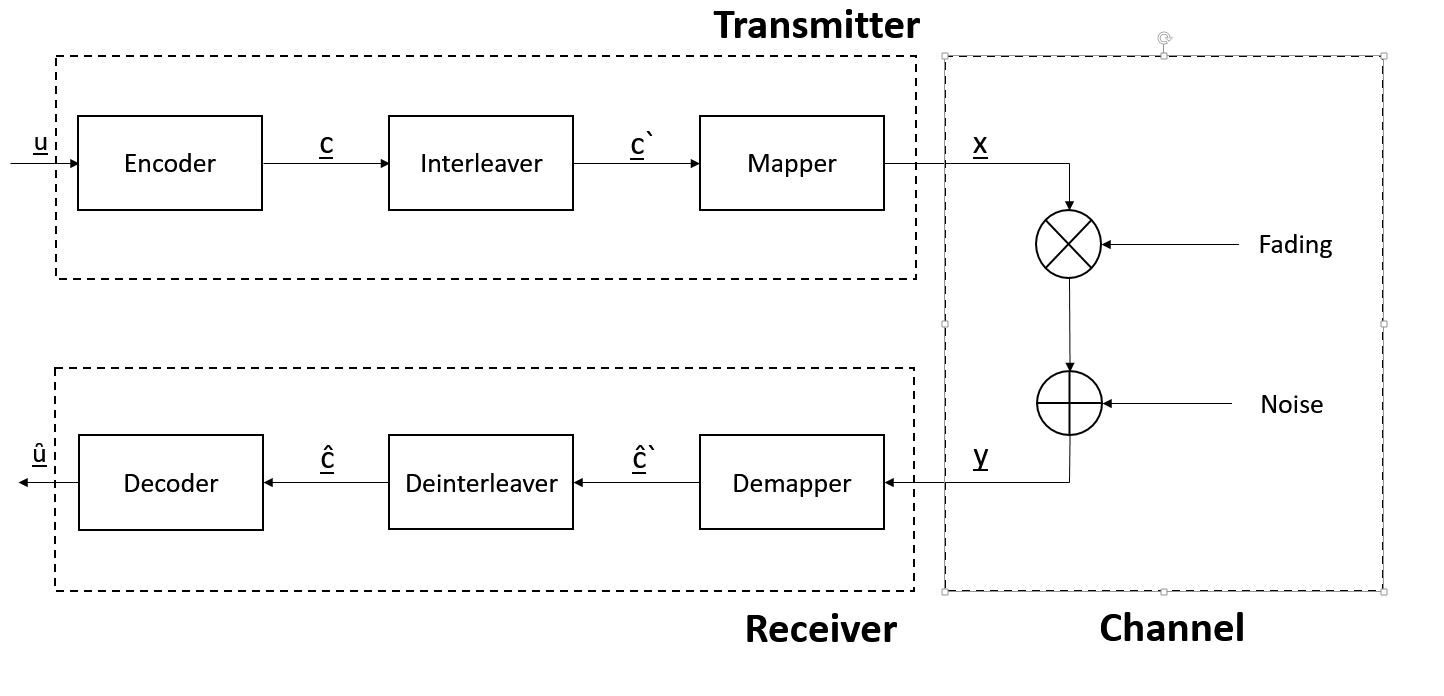
\includegraphics[width=0.7\textwidth]{Channelmodel.PNG}
	\caption{Channelmodel for general Transmitter/Receiver Chain}
	\label{fig:Channelmodel}
\end{figure}
We first start with a small introduction of the system used for all the simulations in the following chapters. We have a few crucial parts of channel blocks needed for every communication link and a few added for improvement in performance or blocks which can be replaced for different approaches. All the blocks were chosen in direct benefit to a LDPC transmission of codewords to make the simulations as simple and effecient as possible. 
Our link is built up in three main blocks: The transmitter, the channel and the receiver. With the transmitter handling the creation of the random codeword, coding with \gls{LDPC} and mapping in different modulation schemes. The channel simulating incoming/existing noise, e.g., \glsl{AWGN}. In the end the receiver will demap and decode our transmitted symbols and compare the decoded bitstream with the initially created codeword.
\newline
The single channel blocks will be explained shortly in the following sections.

\section{Encoder/Decoder}
\label{sec:code};
For our Encoder/Decoder block we will be looking at a WiMax \gls{LDPC} code according to the standard IEEE 802.16e \boldred{cite}. This standard code is used in small and medium distances in urban areas, which fits our model quite well.\boldred{short exp LDPC} While it has heavy computing demands, with the growth of computing power it sees more and more use in everyday use. In our case with WiMax we have different given blocksizes ranging from 576 codewords upto 2304. The rates given are 1/2, 2/3, 3/4, and 5/6. We also only look at coding class A for our simulations. 


\section{Bitinterleave/Deinterleaver}
\label{sec:BIC}
With the help of bitinterleaving we can avoid any kind of "bursterrors", i.e., we avoid any longer blockerrors from malfunctioning transmission of bitstreams for a short period of time. \boldred{Get a paper with interleaving, especially why in LDPC important?}
\newpage

\section{Mapper/Demapper}
\label{sec:mod}

The mapper or modulation is used to assign a specific codelength a symbol which is transmitted. The symbols are located in a real/imaginary plane, also called Inphase/Quadrature Planes (I/Q-Planes). With the distance from the nullpoint of the axis giving us the amplitude of our signal and the angle to the real axis the phase shift. 
There are many forms of modulation schemes, with the most common ones being M-PSK, M-FSK, M-AM and M-QAM. For our simulations we will have a further look in \gls{QPSK}, 16-QAM and 64-QAM, which are depicted below.

\begin{figure}[H]
	\centering
	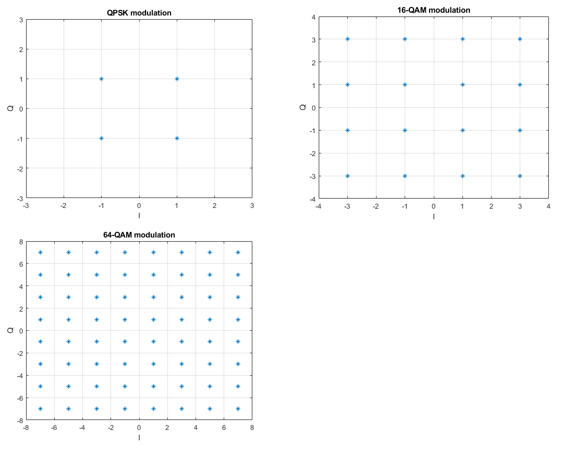
\includegraphics[width=0.95\textwidth]{Modulation_schemes.PNG}
	\caption{Modulation in I/Q planes for QPSK, 16-QAM and 64-QAM}
	\label{fig:Modulation}
\end{figure}

With QPSK the symbols all share the same amplitude and only differ in their respective phase angle. With the information entropy $S = log\textsubscript{2}(M)$\boldred{cite} we can identify the maximum number of bits we can assign in every symbol, with M being the number of symbols in the modulation scheme. So for QPSK the number of bits per symbol amounts to 2.
\newline
With M-QAM, Quadrature Amplitude Modulation, we add the phase shift already implemented into QPSK with the additional differentiation with the amplitude of symbols. For QAM we send signals which differ in their phase shift and also the amplitude.  For 16-QAM we get a maximum of 3 bits per symbols and for 64-QAM 4 bits per symbol.
The modulation schemes make it possible to increase our rate of transmission and is used for any kind of practical transmission of information.

\section{Channel}
\label{sec:channel}
The channel can be modified in many different ways. We can apply different sources of noise or fading, which can relate to realworld interferences. Some interferences experienced in real life transmission are, e.g., thermal noise, distance fading, doppler effect and reflection of signals. To approach those kind of interferences there are many different channel models in simulations, like an \gls{AWGN}-Channel or Rayleigh/Rician fading. We will have a further look into the AWGN-Channel and the Rayleigh fading.
\newline
\boldred{Ausführen, beispiele, bilder}
\subsection{AWGN-Channel}
\boldred{Lookup math}
\newline
The easiest kind of channel manipulation is to add random gaussian noise to the channel, also commonly known as AWGN-Channel. Like the name says we will add noise which is randomly distributed in a gaussian distribution. The probability density function is defined as follows:
\begin{gather*}
f(x|\mu,\sigma^2) = \frac{1}{\sqrt{2\pi\sigma^2}}*e^{-\frac{(x-\mu)^2}{2\mu}}
\end{gather*}
With x being the aquired point, $\mu$ being the mean or expection of the distribution and $\sigma^2$ the variance of the distribution. For our gaussian noise we will take a mean of 0 and a variance of 1, which will simplify further calculations in the following chapters. We will also always look at complex gaussian noise in our simulations. More or less every communication link will have some kind of gaussian noise interference, so we will add the AWGN-Channel to every simulation we run.

\boldred{Add picture of AWGN, pdf or distribution}

\subsection{Rayleigh-Channel}
\boldred{Lookup math}
Another common channel model used in communication theory is Rayleigh fading. Rayleigh fading is used to simulate multipath reception, which means that for a receiver antenna in a wireless link there are many reflected and scattered signals reaching it. This results into construction or destruction of waves. Rayleigh distribution can be defined like this: $R = \sqrt{X^2 + Y^2}$ with X and Y being two independent gaussian distributed random variables. Further calculations will lead to the following pdf:
\begin{gather*}
f(x\sigma) = \frac{1}{\sigma^2}e^{-\frac{x^2}{2\sigma^2}} 
\end{gather*} 

\boldred{Add pictures, spreading, reflection...}
	
\newpage
\chapter{Capacity in an AWGN channel}

We will now look into the maximum capacity we can achieve for our communication model in Chapter 2 with added AWGN noise.

\section{Capacity and Monte-Carlo-Simulation}

In general capacity \textit{C} can be defined as the rate \textit{R} at which information can be reliably transmitted over a channel, which means as long $R \leq \ $C we can achieve a transmission without errors even with noise. All the capacities we wil be looking at will be for complex channel models.

For a AWGN-Channel we will have a simple channel model defined by Y = X + N with X $\sim$ \textit{N}(0,$\sigma\textsubscript{T}^2$) and N $\sim$ \textit{N}(0,1). With this our received signal Y will have a distribution of Y $\sim$ \textit{N}(0,$sigma^2$+1) under the condition that X and N being independently distributed.
We will calculate the capacity as the maximum of mutual information I between X and Y:
\begin{equation}
\label{eq:cap}
C = max(I(X;Y))     
\end{equation}
with X and Y being to independent randomly normal distributed variables.
With the maximum mutual information we calculate the maximum information we can achieve with the given parameters, like modulation, encoding, channel. 
\newline
For the mutual information we can further part it into the differential entropy:
\begin{equation}
I(X;Y) = h(Y) - h(Y|X)
\end{equation}
\newline
With differential entropy being defined as:
\begin{equation}
h(Y) = \int p(y)*[-log(p(y)] \mathrm{d}x
\end{equation}
We will now apply the simulation of monte carlo to turn our integral into an addition. The Monte-Carlo-Simulation will be further explained in the following chapters.
\begin{equation}
h(Y) = h(X+N) = log(\pi*e^{\sigma^2+1}) \quad \textrm{and} \quad h(Y|X) = h(N) = log(\pi*e^{1})
\end{equation}
Further calculations will lead us to the final equation for the capacity in an AWGN-channel:
\begin{equation}
C = log(1+\frac{\sigma^2}{N})
\end{equation}
With this approach we have good approximation values for further calculations with added modulation schemes. It is given that for only AWGN the capacity is at his maximum, there should be no capacity value over the calculated ones here. 

\subsection{Approach in Matlab}
The above mentioned formula 2.4 will be simply implemented in MATLAB. With our noise being randomly distributed around 1 our formula simplifies even more into:
\begin{equation}
\label{eq:AWGN}
C\textsubscript{AWGN} = log(1+SNR) 
\end{equation} 
The SNR here must be transformed into power and not in decibel.

\subsection{Monte-Carlo-Simulation}
Monte Carlo Simulation is widely used in stochastic to get solutions for random experiments. It is used to solve analytical unsolvable problems numerically. MC is based upon the law of large numbers, which says that a large number of performing the same experiment will lead the average of the results close to the expected value. We take this as our bases to get reliable results. The Monte Carlo simulations will be used for two calculations, once already used above for calculating the differential entropy and later once to calculate our theoetical Rayleigh fading curve out of AWGN. 

\section{Capacity for QPSK and M-QAM}
Now we will look into different modulation schemes, which were already mentioned in Chapter~\autoref{sec:mod}. We will implement these modulation schemes into our capacity calculations in an AWGN channel.
\subsection{QPSK}
For QPSK we will have 4 symbols and resulting 2 bits per symbol. Before any simulation or calculation were run we can already be sure that we will not pass the upper bound of 2 bits/Symbol. So the plot will approach the 2 bits/Symbol for high SNR.
After creating a random codeword modulated with the fitting modulation scheme. Noise is added to the signal, which is than received as the bit array Y. The next step to calculate the capacity differs from above. 
\newline
We know that our signal is normal random distributed variables and we have to calculate the differential entropy for h(Y), which is: 
\begin{equation}
\label{eq:entropy}
h(Y) =  \sum_{n=0}^N(-log(p(y\textsubscript{n}))) * \frac{1}{N}
\end{equation} 
with p(y) being the probability of y for a normal distributed variable and N the codelength.
\begin{equation}
p(y) = \frac{1}{n*\pi}*\sum_{i=1}^n(e^{y-x\textsubscript{i}})
\end{equation} 
Here we only need to watch out for the number of symbols in the modulation scheme. For QPSK we have a n = 4, 16-QAM n = 16 and 64-QAM n = 64.
\newline
For the QAM modulation only the above mentioned parameter n must be changed.
 

\subsection{Results}
\begin{figure}[H]
	\centering
	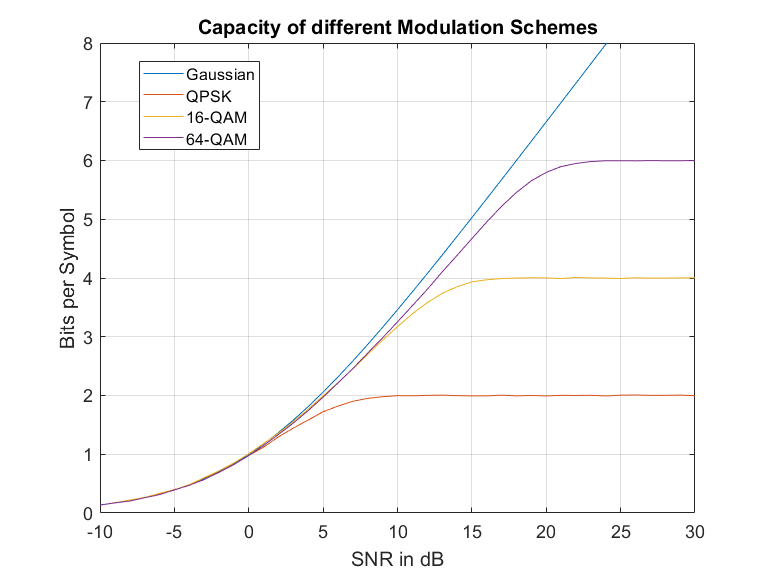
\includegraphics[width=0.7\textwidth]{Capacity_QPSK_QAM.png}
	\caption{Capacity plot for general AWGN-channel, QPSK, 16-QAM and 64-QAM}
	\label{fig:Modulation}
\end{figure}
The results of the calculation in MATLAB can be seen above. We can clearly see the modulated channels approach the desired bit/symbol in a good SNR to bit/symbol rate. The gaussian channel clearly outperforms the modulated channels, clearly seen after 0 dB SNR.

\boldred{Compare with book capactiy!}


\chapter{Transmitter Receiver Chain in MATLAB}

We will now focus in creating a functioning Transmitter-Receiver chain to simulate a wireless communication as real as possible. The blocks for the communication link were shortly introduced in the beginning, but will be explained further in the following chapters. With LDPC WiMax we use a common communication protocol, which simulates a real channel quite well. Furthermore we will use soft mapping to reconstruct our symbols not hard decoding. Later on I will explain my reasoning behind it.  

\section{LDPC and the CML Library}
With a given codeword \textit{x} of length \textit{n} and a generator matrix $G = [I^T|P]$. The parity check matrix texit{H} can now be derived as $H = [-P^T|I\textsubscript{n-k}]$. With the parity check matrix \textit{H} and a code \textit{C} $= xG$ the condition for $cH^t = 0$ must be fulfilled for the codeword to be valid.  
Also with a parity check matrix error correction can be done, that means for single errors we get in our codeword the parity check matrix can selfcorrect our code.
This whole process in MATLAB can be computed with the help of the Coded Modulation Library (CML). For this we have the given function "\textit{InitializeWiMaxLDPC}" to create the parity-check.matrix, "\textit{LdpcEncode}" and "\textit{MpDecode}" to encode and decode our codeword.
We decided on a length of 2304, the maximum length that can be send, and self correcting for 50 iterations to be sure to correct as many errors as possible that we receive at the end of our communication chain.

\section{Soft-demapping vs. Hard-demapping}

These two approaches will result in rather different result in any kind of simulation. We will have a look in both approaches and will compare their unique advantages and disadvantages.
For hard-demapping a received symbol is compared to a given fixed threshhold. At every sampling instant the receiver will decide the state of the bit, either "0" or "1". Hard-demapping uses the minumum Hamming distance to make a decision, which means that bitrow from our receiver is compared to every available constellation point. For every bitdifference between bitrow and constellation point will add to the Hamming distance. In the end the receiver will make a decision by taking the constellation symbol which compared to the created bitrow resembles the most, that means the one with the lowest Hamming distance.
\newline
Major difference to hard-demapping the soft-demapping will use the euclidean distance to make a decision. It will use additional informations supplied by us to make a decision. While hard demapping has no info about the reliability of the receivers decision, soft demapping will gives us exactly this. With the eucladian distance we calculate the distance between received symbol to every constellation point. Furthermore we will use the loglikelihood ratio to calculate the reliability with the euclidian distance.
While hard-demapping is fast and easy to implement in a system it gives us no reliability and as good of performance as soft demapping. In the end it is a decision based on a balance of computing complexity and performance gain.
With many modern systems achieving great computing capability and our desire to create a channel as good as possible we will decide to use soft-demapping. In the next section we will have a further look into soft-demapping and LLR based on a QPSK example.

\begin{figure}[H]
	\centering
	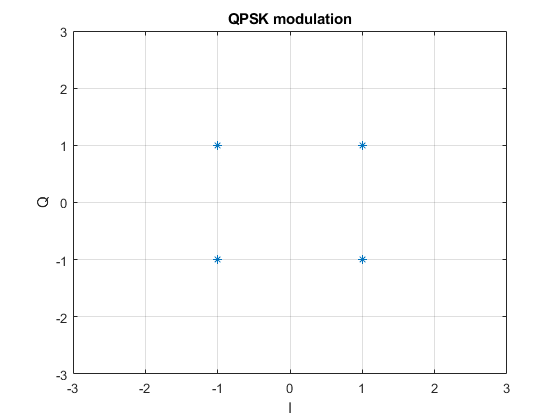
\includegraphics[width=0.7\textwidth]{QPSK.png}
	\caption{Capacity plot for general AWGN-channel, QPSK, 16-QAM and 64-QAM}
	\label{fig:Modulation}
\end{figure}
 
With QPSK we have 4 different symbol constellation also depicted above: (0,0),(0,1),(1,1) and (1,0). The loglikelihood ratio is defined as below

\begin{equation}
\label{eq:llr}
L^n = log\frac{P(Y|B\textsubscript{1} = 0)}{P(Y|B\textsubscript{1} = 1)} = log\frac{P(Y|X\textsubscript{1})+P(Y|X\textsubscript{2})}{P(Y|X\textsubscript{3})+P(Y|X\textsubscript{4})} 
\end{equation} 



\subsection{Results}

After receiving our demodulated symbols we can compare those to our codeword we initially send. With this we will determine the frame errors we got for the whole transmission. A frame is defined as a whole codeword length, that means for us it is 2304 bits sent. We have to simulate at least 100000 of those codewords to receive a reliable error rate. Our error rate = $\frac{\textrm{frame errors}}{\textrm{number of frames sent}}$. With 100 errors being a reliable number we can also prematurely interrupt our simulation after 100 errors to save simulation time.


\section{FER and comparison with capacity plots}

\boldred{Add FER points with respective capacity plots}


\chapter{Communication link for Rayleigh fading channels}

\boldred{Mention slowfading}
We will do the same as before but also add the fading coefficient \textit{H} to our channel. The fading coefficient is represented by rayleigh fading, which was introduced in chapter 2.1... For fading our received signal changes in this way:

\begin{equation}
\label{eq:fading}
Y= \sqrt{\sigma^2}*H*X + N
\end{equation}

With the fading being unknown to our receiver we need a way to extract or estimate the fading coefficient in the channel. An efficient and easy approach to this it to insert a pilot symbol X\textsubscript{p} before the transmission. We also will divide our whole codeword in single blocks T which will range for blocksize equal to one symbol up to the whole codeword being one codeword. For every block we will insert one pilot symbol at the beginning.

\boldred{Graphic for block + pilot}

Our pilot symbol will have the default value of 1, which is also known at the receiver side. This means to estimate the fading we will do this:

\begin{equation}
\label{eq:fadest}
Y_p = \sqrt{\sigma^2}*H*X_p + N
\end{equation}
which leads to:
\begin{equation}
H\textsubscript{est} = \frac{Y_p + N}{\sqrt{\sigma^2} * X_p}
\end{equation}
With this we get a proper estimation for the fading coefficient, but its estimation is highly dependable of the strength of fading and SNR. With higher SNR we receive better estimation not disturbed by the noise as much. And with lesser fading, close to 1, we do not receive a weakened signal, which is hard to distinguish from the noise. 

\boldred{Maybe add graphics which shows the single scenarios}

With the estimated fading coefficient the symbols can be reconstructed.

\begin{equation}
Y\textsubscript{est} = \frac{H}{H\textsubscript{est}}*\sqrt{\sigma^2}*X + \frac{N}{H\textsubscript{est}}
\end{equation}
and with H\textsubscript{est} being close to H we get
\begin{equation}
Y\textsubscript{est} = \sqrt{\sigma^2}*X + \frac{N}{H\textsubscript{est}}
\end{equation}
which can be used to calculate the log likelihood ratio.

\boldred{Maybe add the scatterplot with and w/ rayleigh fading}

\section{Theoratical rayleigh fading FER constructed out of AWGN-Channel}

For a proper simulation we will need a reference to compare our simulation results to. For this we will construct a theoratical FER plot for rayleigh fading out of the AWGN-channel.
First step is the simulate the AWGN channel with the desired codelength over our SNR. In the previous chapters we have already proven that our simulations are match the theoratical curves. With the simulation for AWGN finished we can now start creating
many random value (here n = 10000) rayleigh fading coeffiecients. For every single step of SNR, one step being one SNR, we will compute the SNR after rayleigh fading is created, that means SNR\textsubscript = SNR * H. The SNR for the fading has a corresponding FER-value which we will be add up and divide by the number of fading coefficients.


\begin{equation}
\label{eq:theo}
FER-with-SNRi = \sum_{k = 0}^n FER(SNRi * H(k))
\end{equation}

\boldred{Add plot from AWGN}

It can seen that for the AWGN channel we will reach the error floor really fast at around 3 SNR. For any snr-value which was not simulated for, here only for 0 - 5 SNR, we will add virtual value. While the frame error rate of the AWGN channel reaches a minumum value for high SNR it will never reach 0. In our case we will calculate the theoratical rayleigh FER with error floor 0 and once with error floor $10^{-6}$, just to show the drastic difference in performance with different error floors. Later on we will also prove that the assumend error floor of 
$10^{-6}$ comes close to the real error floor. 

\boldred{Plot for FER with error floor 0 and $10^{-6}$}


\section{Rayleigh fading FER with AWGN channel}


\boldred{Add different plots 1. Simulation with perfect channel knowledge 2. Simulation with estimated coefficient 3. Different blocksizes T=N/2, T=N/16}
\boldred{Explain difference and why?}
We can clearly see a distinct performance difference between the two error floors. OH WOW! SURPRISE!

\section{Increase power of pilot symbol}

\section{Increase of pilot symbols in one block}


\section{Results and comparison with AWGN channel}


\chapter{Conclusion}

\section{Comparison between fading and AWGN channel}

\section{Fazit}




 
















% Generierung des Literaturverzeichnisses
%\bibliography{/path/to/your/.bib/file}

\end{document}
